\documentclass{ximera}

%\usepackage{todonotes}

\newcommand{\todo}{}

\usepackage{esint} % for \oiint
\ifxake%%https://math.meta.stackexchange.com/questions/9973/how-do-you-render-a-closed-surface-double-integral
\renewcommand{\oiint}{{\large\bigcirc}\kern-1.56em\iint}
\fi


\graphicspath{
  {./}
  {ximeraTutorial/}
  {basicPhilosophy/}
  {functionsOfSeveralVariables/}
  {normalVectors/}
  {lagrangeMultipliers/}
  {vectorFields/}
  {greensTheorem/}
  {shapeOfThingsToCome/}
  {dotProducts/}
  {partialDerivativesAndTheGradientVector/}
  {../productAndQuotientRules/exercises/}
  {../normalVectors/exercisesParametricPlots/}
  {../continuityOfFunctionsOfSeveralVariables/exercises/}
  {../partialDerivativesAndTheGradientVector/exercises/}
  {../directionalDerivativeAndChainRule/exercises/}
  {../commonCoordinates/exercisesCylindricalCoordinates/}
  {../commonCoordinates/exercisesSphericalCoordinates/}
  {../greensTheorem/exercisesCurlAndLineIntegrals/}
  {../greensTheorem/exercisesDivergenceAndLineIntegrals/}
  {../shapeOfThingsToCome/exercisesDivergenceTheorem/}
  {../greensTheorem/}
  {../shapeOfThingsToCome/}
  {../separableDifferentialEquations/exercises/}
  {vectorFields/}
}

\newcommand{\mooculus}{\textsf{\textbf{MOOC}\textnormal{\textsf{ULUS}}}}

\usepackage{tkz-euclide}
\usepackage{tikz}
\usepackage{tikz-cd}
\usetikzlibrary{arrows}
\tikzset{>=stealth,commutative diagrams/.cd,
  arrow style=tikz,diagrams={>=stealth}} %% cool arrow head
\tikzset{shorten <>/.style={ shorten >=#1, shorten <=#1 } } %% allows shorter vectors

\usetikzlibrary{backgrounds} %% for boxes around graphs
\usetikzlibrary{shapes,positioning}  %% Clouds and stars
\usetikzlibrary{matrix} %% for matrix
\usepgfplotslibrary{polar} %% for polar plots
\usepgfplotslibrary{fillbetween} %% to shade area between curves in TikZ
%\usetkzobj{all}
\usepackage[makeroom]{cancel} %% for strike outs
%\usepackage{mathtools} %% for pretty underbrace % Breaks Ximera
%\usepackage{multicol}
\usepackage{pgffor} %% required for integral for loops



%% http://tex.stackexchange.com/questions/66490/drawing-a-tikz-arc-specifying-the-center
%% Draws beach ball
\tikzset{pics/carc/.style args={#1:#2:#3}{code={\draw[pic actions] (#1:#3) arc(#1:#2:#3);}}}



\usepackage{array}
\setlength{\extrarowheight}{+.1cm}
\newdimen\digitwidth
\settowidth\digitwidth{9}
\def\divrule#1#2{
\noalign{\moveright#1\digitwidth
\vbox{\hrule width#2\digitwidth}}}




% \newcommand{\RR}{\mathbb R}
% \newcommand{\R}{\mathbb R}
% \newcommand{\N}{\mathbb N}
% \newcommand{\Z}{\mathbb Z}

\newcommand{\sagemath}{\textsf{SageMath}}


%\renewcommand{\d}{\,d\!}
%\renewcommand{\d}{\mathop{}\!d}
%\newcommand{\dd}[2][]{\frac{\d #1}{\d #2}}
%\newcommand{\pp}[2][]{\frac{\partial #1}{\partial #2}}
% \renewcommand{\l}{\ell}
%\newcommand{\ddx}{\frac{d}{\d x}}

% \newcommand{\zeroOverZero}{\ensuremath{\boldsymbol{\tfrac{0}{0}}}}
%\newcommand{\inftyOverInfty}{\ensuremath{\boldsymbol{\tfrac{\infty}{\infty}}}}
%\newcommand{\zeroOverInfty}{\ensuremath{\boldsymbol{\tfrac{0}{\infty}}}}
%\newcommand{\zeroTimesInfty}{\ensuremath{\small\boldsymbol{0\cdot \infty}}}
%\newcommand{\inftyMinusInfty}{\ensuremath{\small\boldsymbol{\infty - \infty}}}
%\newcommand{\oneToInfty}{\ensuremath{\boldsymbol{1^\infty}}}
%\newcommand{\zeroToZero}{\ensuremath{\boldsymbol{0^0}}}
%\newcommand{\inftyToZero}{\ensuremath{\boldsymbol{\infty^0}}}



% \newcommand{\numOverZero}{\ensuremath{\boldsymbol{\tfrac{\#}{0}}}}
% \newcommand{\dfn}{\textbf}
% \newcommand{\unit}{\,\mathrm}
% \newcommand{\unit}{\mathop{}\!\mathrm}
% \newcommand{\eval}[1]{\bigg[ #1 \bigg]}
% \newcommand{\seq}[1]{\left( #1 \right)}
% \renewcommand{\epsilon}{\varepsilon}
% \renewcommand{\phi}{\varphi}


% \renewcommand{\iff}{\Leftrightarrow}

% \DeclareMathOperator{\arccot}{arccot}
% \DeclareMathOperator{\arcsec}{arcsec}
% \DeclareMathOperator{\arccsc}{arccsc}
% \DeclareMathOperator{\si}{Si}
% \DeclareMathOperator{\scal}{scal}
% \DeclareMathOperator{\sign}{sign}


%% \newcommand{\tightoverset}[2]{% for arrow vec
%%   \mathop{#2}\limits^{\vbox to -.5ex{\kern-0.75ex\hbox{$#1$}\vss}}}
% \newcommand{\arrowvec}[1]{{\overset{\rightharpoonup}{#1}}}
% \renewcommand{\vec}[1]{\arrowvec{\mathbf{#1}}}
% \renewcommand{\vec}[1]{{\overset{\boldsymbol{\rightharpoonup}}{\mathbf{#1}}}}

% \newcommand{\point}[1]{\left(#1\right)} %this allows \vector{ to be changed to \vector{ with a quick find and replace
% \newcommand{\pt}[1]{\mathbf{#1}} %this allows \vec{ to be changed to \vec{ with a quick find and replace
% \newcommand{\Lim}[2]{\lim_{\point{#1} \to \point{#2}}} %Bart, I changed this to point since I want to use it.  It runs through both of the exercise and exerciseE files in limits section, which is why it was in each document to start with.

% \DeclareMathOperator{\proj}{\mathbf{proj}}
% \newcommand{\veci}{{\boldsymbol{\hat{\imath}}}}
% \newcommand{\vecj}{{\boldsymbol{\hat{\jmath}}}}
% \newcommand{\veck}{{\boldsymbol{\hat{k}}}}
% \newcommand{\vecl}{\vec{\boldsymbol{\l}}}
% \newcommand{\uvec}[1]{\mathbf{\hat{#1}}}
% \newcommand{\utan}{\mathbf{\hat{t}}}
% \newcommand{\unormal}{\mathbf{\hat{n}}}
% \newcommand{\ubinormal}{\mathbf{\hat{b}}}

% \newcommand{\dotp}{\bullet}
% \newcommand{\cross}{\boldsymbol\times}
% \newcommand{\grad}{\boldsymbol\nabla}
% \newcommand{\divergence}{\grad\dotp}
% \newcommand{\curl}{\grad\cross}
%\DeclareMathOperator{\divergence}{divergence}
%\DeclareMathOperator{\curl}[1]{\grad\cross #1}
% \newcommand{\lto}{\mathop{\longrightarrow\,}\limits}

% \renewcommand{\bar}{\overline}

\colorlet{textColor}{black}
\colorlet{background}{white}
\colorlet{penColor}{blue!50!black} % Color of a curve in a plot
\colorlet{penColor2}{red!50!black}% Color of a curve in a plot
\colorlet{penColor3}{red!50!blue} % Color of a curve in a plot
\colorlet{penColor4}{green!50!black} % Color of a curve in a plot
\colorlet{penColor5}{orange!80!black} % Color of a curve in a plot
\colorlet{penColor6}{yellow!70!black} % Color of a curve in a plot
\colorlet{fill1}{penColor!20} % Color of fill in a plot
\colorlet{fill2}{penColor2!20} % Color of fill in a plot
\colorlet{fillp}{fill1} % Color of positive area
\colorlet{filln}{penColor2!20} % Color of negative area
\colorlet{fill3}{penColor3!20} % Fill
\colorlet{fill4}{penColor4!20} % Fill
\colorlet{fill5}{penColor5!20} % Fill
\colorlet{gridColor}{gray!50} % Color of grid in a plot

\newcommand{\surfaceColor}{violet}
\newcommand{\surfaceColorTwo}{redyellow}
\newcommand{\sliceColor}{greenyellow}




\pgfmathdeclarefunction{gauss}{2}{% gives gaussian
  \pgfmathparse{1/(#2*sqrt(2*pi))*exp(-((x-#1)^2)/(2*#2^2))}%
}


%%%%%%%%%%%%%
%% Vectors
%%%%%%%%%%%%%

%% Simple horiz vectors
\renewcommand{\vector}[1]{\left\langle #1\right\rangle}


%% %% Complex Horiz Vectors with angle brackets
%% \makeatletter
%% \renewcommand{\vector}[2][ , ]{\left\langle%
%%   \def\nextitem{\def\nextitem{#1}}%
%%   \@for \el:=#2\do{\nextitem\el}\right\rangle%
%% }
%% \makeatother

%% %% Vertical Vectors
%% \def\vector#1{\begin{bmatrix}\vecListA#1,,\end{bmatrix}}
%% \def\vecListA#1,{\if,#1,\else #1\cr \expandafter \vecListA \fi}

%%%%%%%%%%%%%
%% End of vectors
%%%%%%%%%%%%%

%\newcommand{\fullwidth}{}
%\newcommand{\normalwidth}{}



%% makes a snazzy t-chart for evaluating functions
%\newenvironment{tchart}{\rowcolors{2}{}{background!90!textColor}\array}{\endarray}

%%This is to help with formatting on future title pages.
\newenvironment{sectionOutcomes}{}{}



%% Flowchart stuff
%\tikzstyle{startstop} = [rectangle, rounded corners, minimum width=3cm, minimum height=1cm,text centered, draw=black]
%\tikzstyle{question} = [rectangle, minimum width=3cm, minimum height=1cm, text centered, draw=black]
%\tikzstyle{decision} = [trapezium, trapezium left angle=70, trapezium right angle=110, minimum width=3cm, minimum height=1cm, text centered, draw=black]
%\tikzstyle{question} = [rectangle, rounded corners, minimum width=3cm, minimum height=1cm,text centered, draw=black]
%\tikzstyle{process} = [rectangle, minimum width=3cm, minimum height=1cm, text centered, draw=black]
%\tikzstyle{decision} = [trapezium, trapezium left angle=70, trapezium right angle=110, minimum width=3cm, minimum height=1cm, text centered, draw=black]


\title{Shifted Theory}

\begin{document}

\begin{abstract}
the shifted story
\end{abstract}
\maketitle





Shifted Exponential Functions are functions that can be represented with formulas of the form

\[
ShExp(x) = A \, r^{B \, x + C} + D
\]



Shifted exponential functions are not exponential functions.  Equal changes in the domain do not give equal percentage changes in the function. \\



As an example, consider $f(x) = 2^{x} + 1$. \\


$f(0) = 1$, $f(1) = 3$, and $f(2) = 5$. \\

The change in the domain from $0$ to $1$ is $1$.  The change from $1$ to $2$ is also $1$. The same change in the domain.

Let's now compare the percentage changes in the function values. \\



\[
\frac{f(1) - f(0)}{f(0)} = \frac{3 - 1}{1} = 2
\]

That is a $200\%$ change in the function value. \\





\[
\frac{f(2) - f(1)}{f(1)} = \frac{5 - 3}{3} = \frac{2}{3}
\]

That is a $66\%$ change in the function value. \\




Equal changes in the domain do not give equal percentage changes in the function values.   These are not exponential functions.


\begin{center}
\textbf{But they are really really really close.} \\
\end{center}


The behavior of shifted exponential function is the same as for exponential functions.  They just exhibit this behavior away from $0$ (the horizontal axis).\\




















\begin{example}  



Analyze   $f(x) = \frac{1}{3} \cdot \, 2^{x+5} - 7$ \\



Categorize:   $f(x) = \frac{1}{3} \cdot \, 2^{x+5} - 7$ is a shifted exponential function, since it matches our template, $A \, r^{B \, x + C} + D$



Let's think about the pieces of the formula to help write our analysis. \\

\begin{idea}




Compared to a basic exponential function graph, where the horizontal axis is the horizontal asymptote, here, the horizontal asymptote has been moved down $\answer{7}$ units, because the constant term in the formula is $-7$.



The ``inside'' (the argument) of the formula for $f(x)$, representing the domain, is $x+5$.  This equals $0$, when $x=-5$.  The exponent is positive for $x>-5$, and because the base is $2 > 1$, this is the direction (right) of unbounded growth.  Therefore, the other direction (left) is where the horizontal asymptote is in effect.  Since the leading coefficient is $\frac{1}{3} > 0$, the unbounded growth is positive.

At $x=-5$, we have our one anchor point for the graph.  The point is $\left(-5, \frac{1}{3} - 7 \right)$, which is $\frac{1}{3}$ above the horizontal asymptote, $y = -7$.


Graph of $y = f(x)$.

\begin{image}
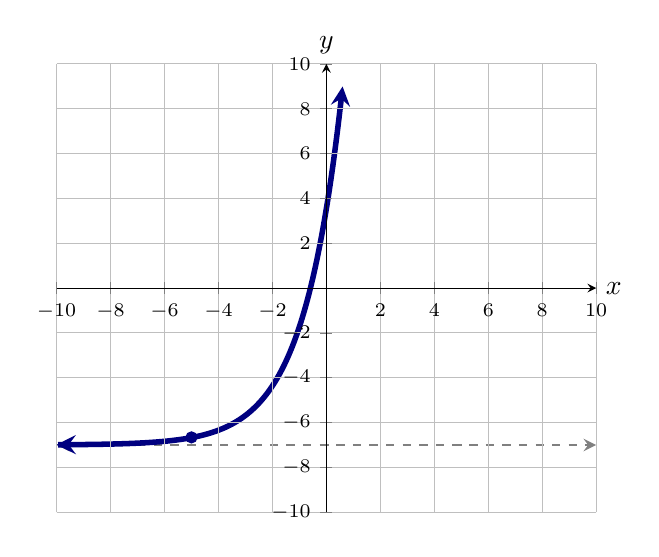
\begin{tikzpicture}
  \begin{axis}[
            domain=-10:10, ymax=10, xmax=10, ymin=-10, xmin=-10,
            axis lines =center, xlabel=$x$, ylabel=$y$, grid = major,
            ytick={-10,-8,-6,-4,-2,2,4,6,8,10},
          	xtick={-10,-8,-6,-4,-2,2,4,6,8,10},
          	ticklabel style={font=\scriptsize},
            every axis y label/.style={at=(current axis.above origin),anchor=south},
            every axis x label/.style={at=(current axis.right of origin),anchor=west},
            axis on top
          ]
          
          \addplot [line width=1, gray, dashed,samples=200,domain=(-10:10),<->] {-7};

      	  \addplot [line width=2, penColor, smooth,samples=200,domain=(-10:0.6),<->] {0.33 * 2^(x+5)-7};

      	  \addplot[color=penColor,fill=penColor,only marks,mark=*] coordinates{(-5,-6.66)};

          


 

  \end{axis}
\end{tikzpicture}
\end{image}




With these ideas, we can write an algebraic analysis.




\end{idea}












\textbf{Domain:} 

The domain of every shifted exponential function is $(-\infty, \infty)$. \\



\textbf{Zeros:}  



$f(x) = \frac{1}{3} \cdot \, 2^{x+5} - 7 = 0$ \\


\begin{align*}
\frac{1}{3} \cdot \, 2^{x+5} - 7 & = 0 \\
\frac{1}{3} \cdot \, 2^{x+5} & = 7 \\
2^{x+5} & = 21 \\
x+5 & = \log_2{21} \\
x & = \log_2{21} - 5
\end{align*}

\textbf{Note:}  $\log_2{21} - 5 \approx -0.607$, which agrees with the graph. \\




\textbf{Continuity:}  

Shifted exponential functions are continuous.  \\








\textbf{Behavior:} 

Like exponential functions, shifted exponential functions are always increasing or always decreasing. \\



The leading coefficient of $f$ is $\frac{1}{3}$, which is positive. \\

The base of $f$ is $2 > 1$.\\

The leading coefficient of the argument is $1$, which is also positive.  



Comparing to $e^x$, a base of $2$ does not change the behavior. A positive leading coefficient does not chnage the behavior.  A positive leading coefficient for the linear exponent does not change the behavior.  We have an increasing function. \\






\textbf{End-Behavior:} 



The negative direction is the direction that makes the exponent negative.  Since the base is $2 > 1$, that makes this the direction that the function value levels off to the constant term, $-7$. 

\[
\lim\limits_{x \to -\infty} f(x) = -7
\]




The other direction is where the shifted exponential function is uunbounded.  Since the leading coefficient of $f$ is positive, $f$ is unbounded positively. \\



\[
\lim\limits_{x \to \infty} f(x) = \infty
\]







\textbf{Global Extrema:} 

Shifted exponential functions do not have global maximums or minimums. \\


\textbf{Local Extrema:} 

Shifted exponentials function do not have local maximums or minimums. \\



\textbf{Range:} The end-behavior tells us that the range is $(-7, \infty)$.





\end{example}




















\begin{example}  Another View



$f(x) = \frac{1}{3} \, 2^{x+5} - 7$ is the function in the last example.  We could take advantage of exponential algebra to simplify the formula.   \\

\[ 
f(x) = \frac{1}{3} \, 2^{x+5} - 7 = \frac{1}{3} \, 2^x \cdot 2^5 - 7 = \frac{32}{3} \, 2^x  - 7
\]


We now have a basic exponential function shifted down $7$.  The new base is still $2$ and the new leading coefficient is $\frac{32}{3}$.





By doing this, we change our strategic point to $\left( 0, \frac{32}{3} - 7 \right) = \left( 0, \frac{11}{3} \right)$.




\begin{image}
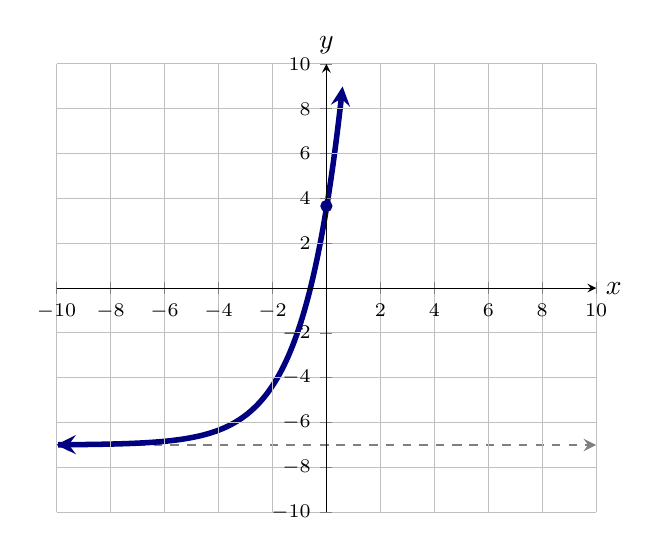
\begin{tikzpicture}
  \begin{axis}[
            domain=-10:10, ymax=10, xmax=10, ymin=-10, xmin=-10,
            axis lines =center, xlabel=$x$, ylabel=$y$, grid = major,
            ytick={-10,-8,-6,-4,-2,2,4,6,8,10},
            xtick={-10,-8,-6,-4,-2,2,4,6,8,10},
            ticklabel style={font=\scriptsize},
            every axis y label/.style={at=(current axis.above origin),anchor=south},
            every axis x label/.style={at=(current axis.right of origin),anchor=west},
            axis on top
          ]
          
          \addplot [line width=1, gray, dashed,samples=200,domain=(-10:10),<->] {-7};

          \addplot [line width=2, penColor, smooth,samples=200,domain=(-10:0.6),<->] {0.33 * 2^(x+5)-7};

          \addplot[color=penColor,fill=penColor,only marks,mark=*] coordinates{(0,3.66)};

          


 

  \end{axis}
\end{tikzpicture}
\end{image}




\end{example}






















\begin{example} Altering Algebraically



Let $G(t) = 4 \cdot 3^{2t-1} - 5$.  

We could take advantage of exponential algebra to simplify the exponent.   \\

\[ 
G(t) = 4 \cdot 3^{2t-1} - 5 = 4 \cdot 3^{2t} \cdot \frac{1}{3} - 5 = \frac{4}{3} \cdot (3^2)^t - 5  = \frac{4}{3} \cdot 9^t - 5
\]


We now have a basic exponential function shifted down $\answer{5}$.  The new base is $\answer{9}$ and the new leading coefficient is $\answer{\frac{4}{3}}$.




The leading coefficient is $\frac{4}{3} > 0$ and the base is $9 > 1$. Therefore, $G(t)$ is an increasing function.  The function values will be positive, once they overcome the drop of $5$ to the horizontal asymptote.



$G(t) = \frac{4}{3} \cdot 9^t - 5$ is a transformation of $g(t) = 3^t$.  Let's compare $G(t)$ back to $3^t$.


Since the new base $9$ is greater than the old base of $3$, the function grows faster.  The graph goes up to the right faster and steeper.  This means the graph is compressed horizontally, which is the result of multiplying by $2$ in the exponent.





End-Behavior:
\[
\lim\limits_{t \to -\infty}G(t) = \answer{-5}  
\]

\[
\lim\limits_{t \to \infty}G(t) = \answer{\infty}
\]




\end{example}




























\begin{example}  



Analyze   $B(t) = -2 \, \left( \frac{2}{3} \right)^{3-t} + 4$ \\


Categorize: $B(t) = -2 \, \left( \frac{2}{3} \right)^{3-t} + 4$ is a shifted exponential function, becuase it matches our template,  $A \, r^{B \, x + C} + D$. \\

\begin{idea}


\textbf{\textcolor{purple!85!blue}{Formula dissection:}}  \\


$\blacktriangleright$  the base: $\frac{2}{3} < 1$\\
$\blacktriangleright$  the linear exponent: $3-t$ is positive for large negative $t$. \\
$\blacktriangleright$  the linear exponent: $3-t$ is negative for large positive $t$. \\
$\blacktriangleright$  the leading coefficient is negative. \\


Together, these tell us that $B(t)$ settles down for large negative $t$ and that $B(t)$ becomes unbounded when $t$ is large and positive.



This is a transformed version of the basic exponential function template $\left( \frac{2}{3} \right)^{-t} = \left( \answer{\frac{3}{2}} \right)^t$.  



When $t < 0$, then $-t > 0$ and we get  $\left( \frac{2}{3} \right)^{positive}$ and the basic exponential portion is becoming smaller, approaching $0$.  





\[ \lim\limits_{t \to -\infty} \left( \frac{2}{3} \right)^{-t}  = 0 \]



When $t > 0$, then $-t < 0$ and we get  $\left( \frac{2}{3} \right)^{negative} = \left( \frac{3}{2} \right)^{positive}$ and $B(t)$ is becoming unbounded.  



\[ \lim\limits_{t \to \infty} \left( \frac{2}{3} \right)^{-t}  = \lim\limits_{t \to \infty} \left( \frac{3}{2} \right)^t  = \infty \]




Exponential growth to the right and decay to the left.






Since $a = -2 < 0$, these smaller/larger values of $-2 \, \left( \frac{2}{3} \right)^{-t}$ are smaller/larger negative values.



We also have two shifts. One from the $3$ in the exponent and the second from the constant term, $4$:




$\blacktriangleright$ \textbf{Vertical Shift}


Adding $4$ to the outside shifts the graph vertically up $4$.  The asymptote is $y = 4$ and 

\[ \lim\limits_{t \to -\infty} B(t) = 4 \]



$\blacktriangleright$ \textbf{Horizontal Shift}

Our exponent here is $3 - t$.  Our function's exponent is zero, $3-t=0$ when $t=3$. Our one anchor point is shifted over to $3$.  Multipying by $-2$, means the dot is $2$ away(below) from the horizontal asymptote, which is now $y=4$.  Our anchor point is $(3, 2)$.








Graph of $y = B(t)$.

\begin{image}
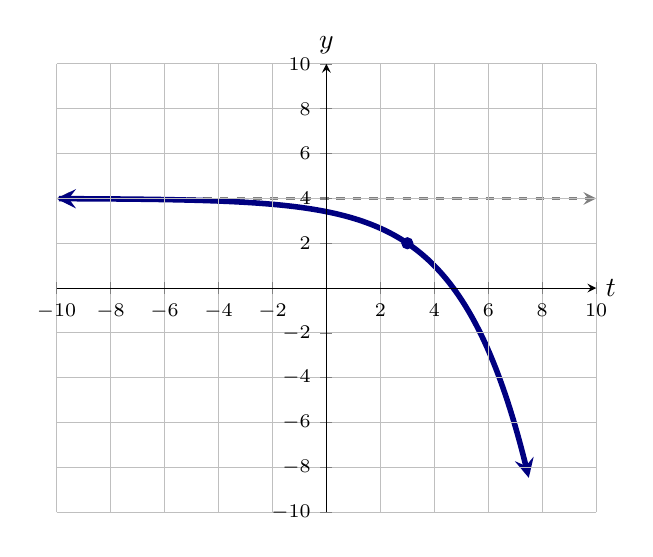
\begin{tikzpicture}
  \begin{axis}[
            domain=-10:10, ymax=10, xmax=10, ymin=-10, xmin=-10,
            axis lines =center, xlabel=$t$, ylabel=$y$, grid = major,
            ytick={-10,-8,-6,-4,-2,2,4,6,8,10},
          	xtick={-10,-8,-6,-4,-2,2,4,6,8,10},
          	ticklabel style={font=\scriptsize},
            every axis y label/.style={at=(current axis.above origin),anchor=south},
            every axis x label/.style={at=(current axis.right of origin),anchor=west},
            axis on top
          ]
          
          \addplot [line width=1, gray, dashed,samples=200,domain=(-10:10),<->] {4};

      	  \addplot [line width=2, penColor, smooth,samples=200,domain=(-10:7.5),<->] {-2 * (0.666^(3-x)) + 4};

      	  \addplot[color=penColor,fill=penColor,only marks,mark=*] coordinates{(3,2)};

          


  \end{axis}
\end{tikzpicture}
\end{image}



With these ideas, we can write an algebraic analysis.

\end{idea}











\textbf{Domain:} 

The domain of every shifted exponential function is $(-\infty, \infty)$. \\



\textbf{Zeros:}  



$B(t) = -2 \, \left( \frac{2}{3} \right)^{3-t} + 4$ \\


\begin{align*}
-2 \, \left( \frac{2}{3} \right)^{3-t} + 4 & = 0 \\
-2 \, \left( \frac{2}{3} \right)^{3-t}  & = -4 \\
\left( \frac{2}{3} \right)^{3-t} & = \frac{-4}{-2} = 2 \\
3-t & = \log_{\tfrac{2}{3}}(2)\\
3 - \log_{\tfrac{2}{3}}(2) & = t
\end{align*}

\textbf{Note:}  We'll need to switch bases to use the calculatr=or to get an approximatio to comapre with the graph.



\[
3 - \log_{\tfrac{2}{3}}(2) = 3 - \frac{\ln(2)}{\ln\left( \frac{2}{3}  \right)} \approx 4.709511291  
\]


That agrees with the graph. \\




\textbf{Continuity:}  

Shifted exponential functions are continuous.  \\








\textbf{Behavior:} 

Like exponential functions, shifted exponential functions are always increasing or always decreasing. \\



The leading coefficient of $B$ is $-2$, which is negative. \\

The base of $B$ is $\frac{2}{3} < 1$.\\

The leading coefficient of the linear exponent is $-1$, which is negative.  



Comparing to $e^x$, a base of $-2$ does change the behavior from increasing to decreasing. A negative leading coefficient changes the behavior back to increasing.  A negative leading coefficient for the linear exponent does changes the behavior again to decreasing.  We have an decreasing function. \\






\textbf{End-Behavior:} 



The positive direction is the direction that makes the exponent negative.  Since the base is $\frac{2}{3} < 1$, that makes this the direction that the function value becomes unbounded.  The negative leading coefficient means $B$ is unbounded negatively.



\[
\lim\limits_{t \to \infty} B(t) = -\infty
\]


The other direction is where the shifted exponential function approached the constant term



\[
\lim\limits_{x \to -\infty} f(x) = 4
\]










\textbf{Global Extrema:} 

Shifted exponential functions do not have global maximums or minimums. \\


\textbf{Local Extrema:} 

Shifted exponentials function do not have local maximums or minimums. \\



\textbf{Range:} The end-behavior tells us that the range is $(-\infty, 4)$.










\end{example}


































In the example above, we could have algebraically moved the horizontal shift to the leading coefficient.



\[
-2 \, \left( \frac{2}{3} \right)^{3-t} + 4
\]


\[
-2 \, \left( \frac{2}{3} \right)^{3} \cdot \left( \frac{2}{3} \right)^{-t}+ 4
\]


\[
-2 \, \left( \frac{8}{27} \right)  \cdot \left( \frac{2}{3} \right)^{-t}+ 4
\]


\[
\left( \frac{-16}{27} \right)  \cdot \left( \frac{2}{3} \right)^{-t}+ 4
\]


We could have further transfered the negative sign in the exponent to the base by reciprocating the base.

\[
\left( \frac{-16}{27} \right)  \cdot \left( \frac{3}{2} \right)^t+ 4
\]



Algebra provides many tools for modifying the representing formula and altering how we think about the behavior. \\








\begin{example}  Shifted Exponential Function



Consider  $K(f) = 3^{5-f} - 5$ \\

\begin{question}
 

The base is \wordChoice{\choice{less than}\choice[correct]{greater than}} $1$.
\end{question}
\begin{question}


The exponent gets big and positive when $f$ gets big and \wordChoice{\choice{positive}\choice[correct]{negative}}.
\end{question}
\begin{question}


The graph will become unbounded to the \wordChoice{\choice{right}\choice[correct]{left}}.\\
\end{question}

\begin{question}


The horizontal asymptote is $y = \answer{-5}$.
\end{question}

\begin{question}


The graph will approach the asymptote to the \wordChoice{\choice[correct]{right}\choice{left}}.\\
\end{question}
\begin{question}


Our one strategic anchor point moves to $\left(\answer{5}, \answer{-4}\right)$.
\end{question}
\begin{question}


The graph will become unbounded \wordChoice{\choice[correct]{up}\choice{down}}.\\
\end{question}




Graph of $y = K(f)$.

\begin{image}
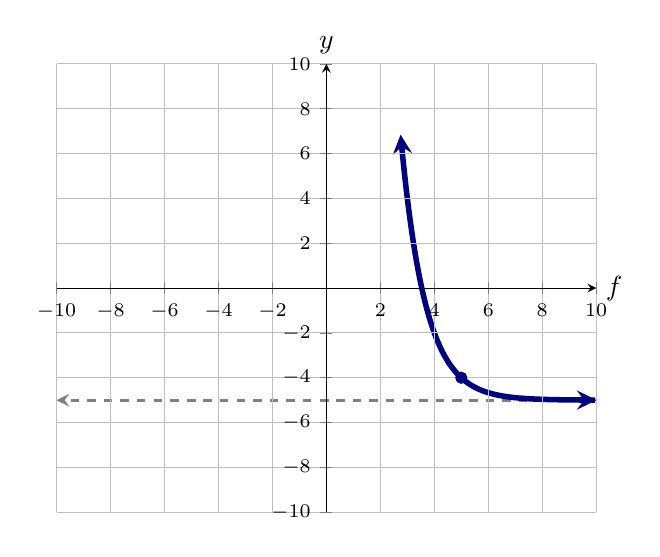
\begin{tikzpicture}
  \begin{axis}[
            domain=-10:10, ymax=10, xmax=10, ymin=-10, xmin=-10,
            axis lines =center, xlabel=$f$, ylabel=$y$, grid = major,
            ytick={-10,-8,-6,-4,-2,2,4,6,8,10},
          	xtick={-10,-8,-6,-4,-2,2,4,6,8,10},
          	ticklabel style={font=\scriptsize},
            every axis y label/.style={at=(current axis.above origin),anchor=south},
            every axis x label/.style={at=(current axis.right of origin),anchor=west},
            axis on top
          ]
          
          \addplot [line width=1, gray, dashed,samples=200,domain=(-10:10),<->] {-5};

      	  \addplot [line width=2, penColor, smooth,samples=200,domain=(2.75:10),<->] {3^(5-x) - 5};

      	  \addplot[color=penColor,fill=penColor,only marks,mark=*] coordinates{(5,-4)};

 

  \end{axis}
\end{tikzpicture}
\end{image}





Quick ideas: \\

\begin{itemize}
\item The natural or implied domain of $K$ is $\mathbb{R}$.
\item $K$ is always decreasing.
\item $K$ has no maximums or minimums.
\item $\lim\limits_{f \to -\infty} K(f) = \infty$
\item $\lim\limits_{f \to \infty} K(f) = -5$
\end{itemize}


\end{example}





















\begin{center}
\textbf{\textcolor{green!50!black}{ooooo-=-=-=-ooOoo-=-=-=-ooooo}} \\

more examples can be found by following this link\\ \link[More Examples of Exponential Functions]{https://ximera.osu.edu/csccmathematics/precalculus2/precalculus2/expFunctions/examples/exampleList}

\end{center}









\end{document}
